\documentclass[a4paper]{article} 
\addtolength{\hoffset}{-2.25cm}
\addtolength{\textwidth}{4.5cm}
\addtolength{\voffset}{-3.25cm}
\addtolength{\textheight}{5cm}
\setlength{\parskip}{0pt}
\setlength{\parindent}{0in}

%----------------------------------------------------------------------------------------
%	PACKAGES AND OTHER DOCUMENT CONFIGURATIONS
%----------------------------------------------------------------------------------------
\usepackage{blindtext} % Package to generate dummy text
\usepackage{charter} % Use the Charter font
\usepackage[utf8]{inputenc} % Use UTF-8 encoding
\usepackage{microtype} % Slightly tweak font spacing for aesthetics
\usepackage[english, ngerman]{babel} % Language hyphenation and typographical rules
\usepackage{amsthm, amsmath, amssymb} % Mathematical typesetting
\usepackage{float} % Improved interface for floating objects
\usepackage[final, colorlinks = true, 
            linkcolor = black, 
            citecolor = black]{hyperref} % For hyperlinks in the PDF
\usepackage{graphicx, multicol} % Enhanced support for graphics
\usepackage{xcolor} % Driver-independent color extensions
\usepackage{marvosym, wasysym} % More symbols
\usepackage{rotating} % Rotation tools
\usepackage{censor} % Facilities for controlling restricted text
\usepackage{listings, style/lstlisting} % Environment for non-formatted code, !uses style file!
\usepackage{pseudocode} % Environment for specifying algorithms in a natural way
\usepackage{style/avm} % Environment for f-structures, !uses style file!
\usepackage{booktabs} % Enhances quality of tables
\usepackage{tikz-qtree} % Easy tree drawing tool
\tikzset{every tree node/.style={align=center,anchor=north},
         level distance=2cm} % Configuration for q-trees
\usepackage{style/btree} % Configuration for b-trees and b+-trees, !uses style file!
\usepackage[backend=biber,style=numeric,
            sorting=nyt]{biblatex} % Complete reimplementation of bibliographic facilities
\addbibresource{ecl.bib}
\usepackage{csquotes} % Context sensitive quotation facilities
\usepackage[yyyymmdd]{datetime} % Uses YEAR-MONTH-DAY format for dates
\renewcommand{\dateseparator}{-} % Sets dateseparator to '-'
\usepackage{fancyhdr} % Headers and footers
\pagestyle{fancy} % All pages have headers and footers
\fancyhead{}\renewcommand{\headrulewidth}{0pt} % Blank out the default header
\fancyfoot[L]{} % Custom footer text
\fancyfoot[C]{} % Custom footer text
\fancyfoot[R]{\thepage} % Custom footer text
\newcommand{\note}[1]{\marginpar{\scriptsize \textcolor{red}{#1}}} % Enables comments in red on margin

%----------------------------------------------------------------------------------------

\begin{document}

%-------------------------------
%	TITLE SECTION
%-------------------------------

\fancyhead[C]{}
\hrule \medskip % Upper rule
\begin{minipage}{0.295\textwidth} 
\raggedright
\footnotesize
\begin{figure}[H]
    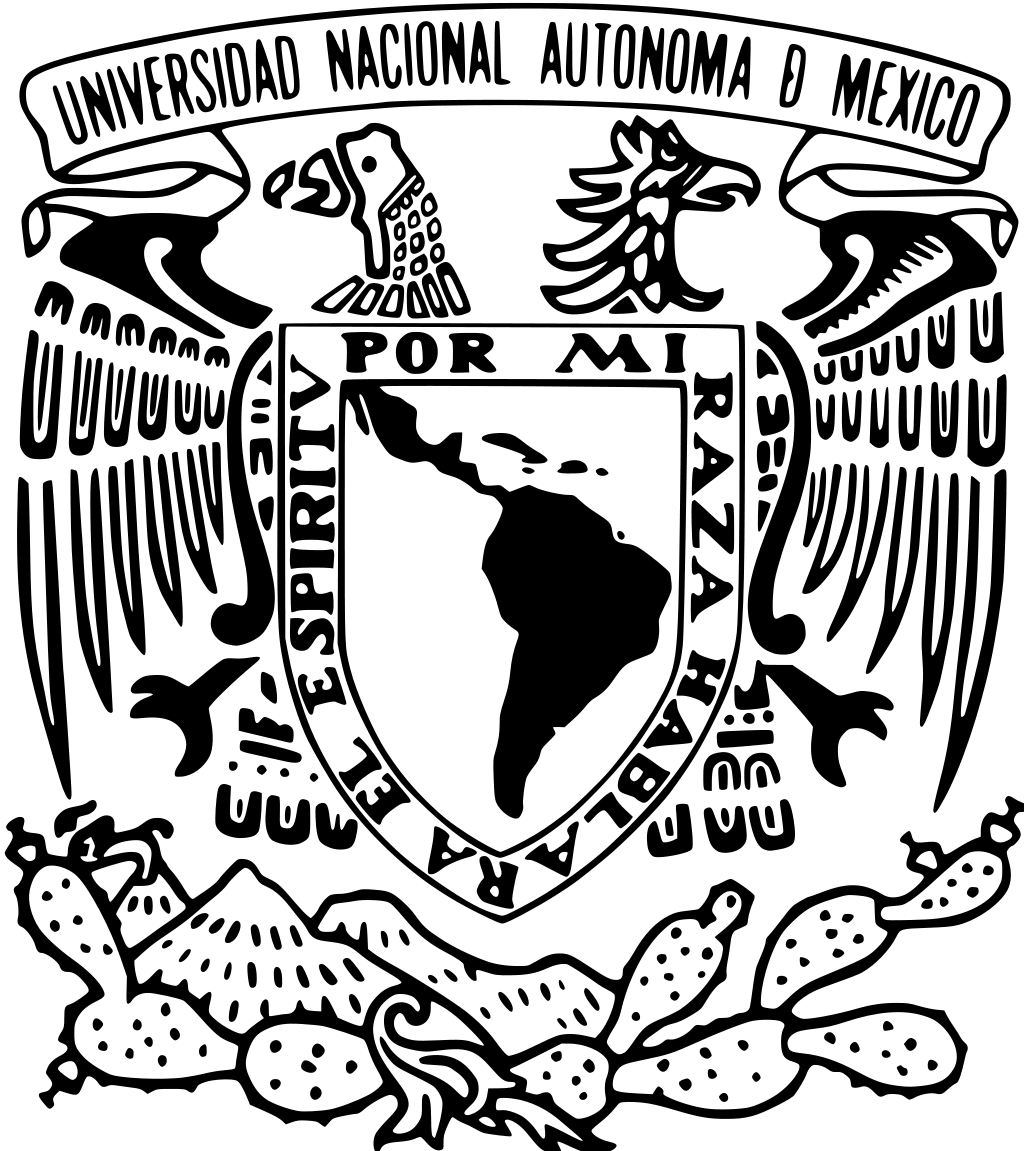
\includegraphics[scale = 0.053]{style/UNAM.png}
\end{figure}
%YOURNAME \hfill\\   
%YOURSTUDENTID\hfill\\
%YOURMAIL
\end{minipage}
\begin{minipage}{0.4\textwidth} 
\centering 
\large 
Lógica Computacional 2022-I\\ 
\normalsize 
Ejercicio semanal 2\\
\normalsize
López Miranda Angel Mauricio
\end{minipage}
\begin{minipage}{0.295\textwidth} 
\raggedleft
\footnotesize
\begin{wrapfigure}{}{\textwidth} %this figure will be at the right
    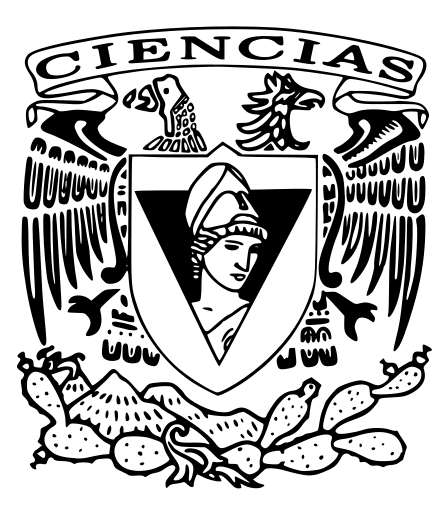
\includegraphics[width=0.4\textwidth]{style/ciencias.png}
\end{wrapfigure}
%\begin{figure}[H]
 %   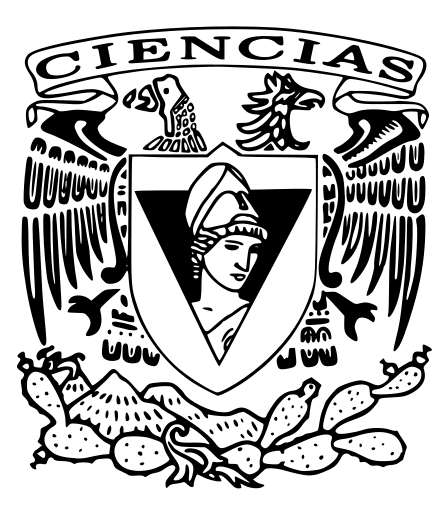
\includegraphics[scale = 0.12]{style/ciencias.png}
%\end{figure}
%\today\hfill\\
\end{minipage}
\medskip\hrule 
\bigskip

%-------------------------------
%	CONTENTS
%-------------------------------

%\section{First Exercise}
%\blindtext
%\subsection{First Subtask}
%Some equations
%\begin{align*}
%y &=  \sum\limits_{i,k} m_i \cdot f^k \\
%x &=  
%\underset{11}{\underbrace{3 + 8}} + 5 + 7
%\end{align*}

%\subsection{Second Subtask}
%\blindtext

%\bigskip

%------------------------------------------------

%\section{Second Exercise}
%\blindtext
%\subsection{First Subtask}

%\bigskip

%------------------------------------------------

\begin{enumerate}
\item Defina recursivamente las siguientes funciones:

	\begin{enumerate}
 		\item {\tt ni} que recibe una fórmula $\varphi$ y regresa el número de símbolos de implicación que tiene la fórmula. Por ejemplo

                  $${\tt ni} (p \land r \to \lnot (q \to r)) = 2$$
                  
        Definamos {\tt ni} de forma recursiva:\\
        ${\tt ni} \varphi=\varphi$\\
        ${\tt ni} \neg\varphi=$ ${\tt ni}(\varphi)$\\
        ${\tt ni} \vartheta \land\varphi=$ ${\tt ni} (\vartheta)+$ ${\tt ni}(\varphi)$\\
        ${\tt ni} \vartheta \lor\varphi=$ ${\tt ni} (\vartheta)+$ ${\tt ni}(\varphi)$\\
        ${\tt ni} \vartheta \to \varphi=$ $1+$ ${\tt ni} (\vartheta)+$ ${\tt ni}(\varphi)$\\
        ${\tt ni} \vartheta \leftrightarrow\varphi=$ ${\tt ni} (\vartheta)+$ ${\tt ni}(\varphi)$\\
        
		\item {\tt nd} que recibe una fórmula $\varphi$ y regresa el número de símbolos de disyunción que tiene la fórmula. Por ejemplo

                  $${\tt nd} (p \lor r \to \lnot (q \lor r) \land (s\lor\neg t)) = 3$$
                  
        Definamos {\tt nd} de forma recursiva:\\
        ${\tt nd} \varphi=\varphi$\\
        ${\tt nd} \neg\varphi=$ ${\tt nd}(\varphi)$\\
        ${\tt nd} \vartheta \land\varphi=$ ${\tt nd} (\vartheta)+$ ${\tt nd}(\varphi)$\\
        ${\tt nd} \vartheta \lor\varphi=$ $1+$ ${\tt nd} (\vartheta)+$ ${\tt nd}(\varphi)$\\
        ${\tt nd} \vartheta \to \varphi=$ ${\tt nd} (\vartheta)+$ ${\tt nd}(\varphi)$\\
        ${\tt nd} \vartheta \leftrightarrow\varphi=$ ${\tt nd} (\vartheta)+$ ${\tt nd}(\varphi)$\\
		\item {\tt qi} que recibe una fórmula y regresa una fórmula en que no figura el símbolo $\to$, usando la equivalencia lógica $A\to B\equiv \neg A\lor B$. Por ejemplo:

		$${\tt qi} (p \land r \to \lnot (q \to r)) = \lnot (p \land r) \lor \lnot(\lnot q \lor r)$$
		
		Definamos {\tt ni} de forma recursiva:\\
        ${\tt qi} \varphi=\varphi$\\
        ${\tt qi} \neg\varphi=$ ${\tt qi}(\varphi)$\\
        ${\tt qi} \vartheta \land\varphi=$ ${\tt qi} (\vartheta)\land$ ${\tt qi}(\varphi)$\\
        ${\tt qi} \vartheta \lor\varphi=$ ${\tt qi} (\vartheta)\lor$ ${\tt qi}(\varphi)$\\
        ${\tt qi} \vartheta \to \varphi=$ $\neg$ ${\tt qi} (\vartheta)\lor$ ${\tt qi}(\varphi)$\\
        ${\tt qi} \vartheta \leftrightarrow\varphi=$ ${\tt ni} (\vartheta)\leftrightarrow$ ${\tt qi}(\varphi)$\\
	\end{enumerate}
	\item Utilizando las definiciones anteriores demuestre mediante inducción estructural que para cualquier fórmula $\varphi$, se cumple:

	$${\tt nd}({\tt qi}\,(\varphi)) = {\tt nd}(\varphi) + {\tt ni}(\varphi)$$

\end{enumerate}

\end{document}

\end{document}
